\documentclass[pdf]{beamer}
\usepackage{listings}
\usepackage{color}

\definecolor{dkgreen}{rgb}{0,0.6,0}
\definecolor{gray}{rgb}{0.5,0.5,0.5}
\definecolor{mauve}{rgb}{0.58,0,0.82}

\lstset{frame=none,
language=C,
columns=flexible,
numberstyle=\tiny\color{gray},
keywordstyle=\color{blue},
commentstyle=\color{dkgreen},
stringstyle=\color{mauve},
breaklines=true,
breakatwhitespace=true,
tabsize=4,
showstringspaces=false,
basicstyle=\ttfamily
}
\usepackage{parskip}
\usepackage{graphicx}
\graphicspath{{../images/}}

\mode<presentation>
{
	\usetheme{default}      % or try Darmstadt, Madrid, Warsaw, ...
	\usecolortheme{default} % or try albatross, beaver, crane, ...
	\usefonttheme{default}  % or try serif, structurebold, ...
	\setbeamertemplate{navigation symbols}{}
	\setbeamertemplate{caption}[numbered]
}

\begin{document}
\title{Intel Cloud Orchestration Networking Design and Goals}
\author{Matthew Johnson, Cody Malick, and Garrett Smith}
\date{17 February, 2017}

\maketitle
\begin{frame}
	\frametitle{Table of Contents}
	\tableofcontents
\end{frame}

\begin{frame}
	\frametitle{Team Cloud Orchestra}
	\section{Introduction}
	Our team is implementing a software defined network based on Open
	vSwitch for a cloud orchestration technology called Ciao.

	Our client is Rob Nesius, Engineering Manager at Intel Corporation.
\end{frame}

\begin{frame}
	\frametitle{Scope}
	\section{Scope}
	What is a cloud?
	\begin{figure}[H]
		\caption{The Cloud - Randall Munroe~\cite{xkcd908}}
		\begin{center}
			%\makebox[\textwidth]{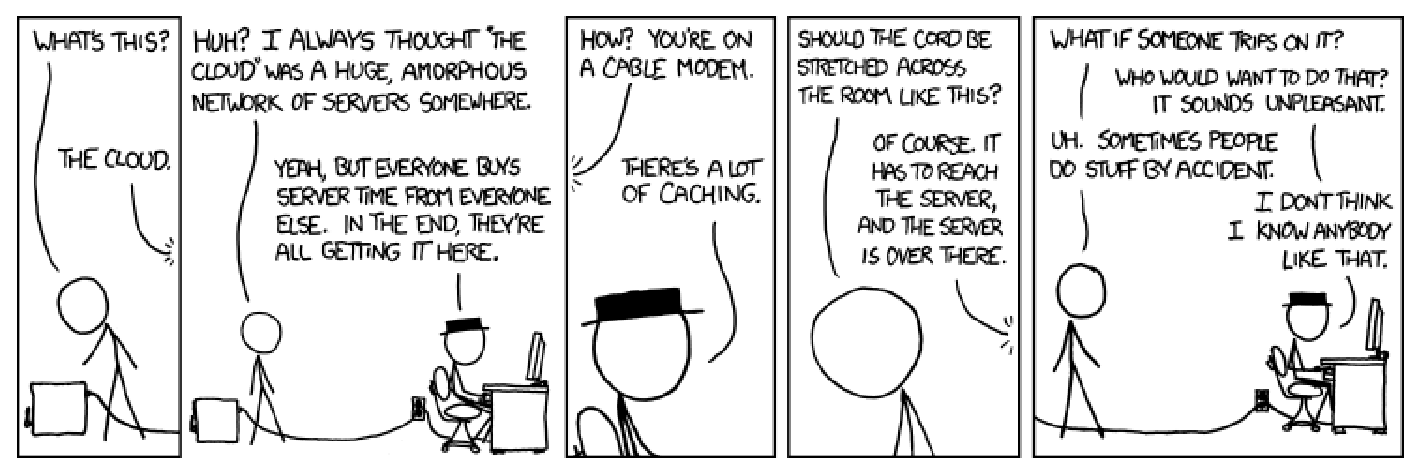
\includegraphics[width=\textwidth]{xkcd.eps}}
		\end{center}
	\end{figure}

	"A huge, amorphous network of servers somewhere"

\end{frame}

\begin{frame}
	\frametitle{Scope}
	The network connecting the nodes must be controlled. In our case, this
	is achieved by the Cloud Integrated Advanced Orchestrator, or Ciao.

	Ciao provides an easy to deploy, secure, scalable cloud orchestration
	system which handles virtual machines, containers, and bare metal apps
	agnostically as generic workloads~\cite{ciao}.
\end{frame}

\begin{frame}
	\frametitle{Scope}
	The servers, or nodes, in these clouds need to talk to each other, hence
	the need for a network solution.

	Ciao uses a software defined network to allow different compute nodes to
	communicate with each other.

	Software defined networking is a software abstraction of physical
	networking solutions, allowing for ``a more scalable and centralized
	network control architecture''~\cite{goransson}.
\end{frame}

\begin{frame}
	\frametitle{Project Goals}
	\framesubtitle{Goal One}
	\section{Project Goals}
	Switch Ciao Generic Routing Encapsulation (GRE) tunnel implementation to
	use Open vSwitch-created GRE tunnels.

	\begin{description}[style=nextline]
		\item[Generic Routing Encapsulation (GRE)]
			GRE encapsulates an arbitrary network layer protocol so
			it can be sent over arbitrary network layer
			protocol~\cite{rfc1701}.
		\item[Open vSwitch (OVS)]
			Open vSwitch is a ``multilayer virtual switch\ldots
			designed to enable massive network automation through
			programmatic extension''~\cite{ovs}.
	\end{description}
\end{frame}

\begin{frame}
	\frametitle{Project Goals}
	\framesubtitle{Goal Two}
	Switch the tunneling protocol implementation to best-performing network
	virtualization technology based on our performance measurement of each
	on data center network cards.
\end{frame}

\begin{frame}
	\frametitle{Project Goals}
	\framesubtitle{Goal Three (optional)}
	Replace the Linux bridge implementation with OVS switch instances.
\end{frame}

\begin{frame}
	\frametitle{Project Design}
	\section{Project Design}
	\subsection{Open vSwitch Database Management Protocol}

	Open vSwitch uses a database to manage configuration while running.
	The configuration can be updated on the fly by accessing its management
	protocol using the Open vSwitch Database Management Protocol, defined
	in RFC 7047\cite{rfc7047}
\end{frame}

\begin{frame}[fragile]
	\frametitle{OVS Database Management Protocol}
	One of the main goals of the project is to implement OVS built network
	bridges programmatically. The protocol uses JSON to build its commands.
	\\
	\begin{lstlisting}[caption=Example insert OVS DB Management Protocol]
	{
	  "op": "insert",
	  "table": "Bridge",
	  "row": 2,
	  "uuid-name": 00000000-0000-0000-0000-000000000000
	}
	\end{lstlisting}
\end{frame}

\begin{frame}[fragile]
	\frametitle{Libovsdb}
	\subsection{libovsdb}
	Libovsdb is an open source library that provides a Go programming
	language wrapper around the OVS Database Management Protocol. This tool
	is quite helpful because it allows us easy access to the Management
	Protocol, without having to manually create JSON. Here is
	an example:\cite{gosample} \\

\begin{lstlisting}[caption=Example insert operation using libovsdb]
	// simple insert operation
	insertOp := libovsdb.Operation{
	    Op:	  "insert",
	    Table:	  "Bridge",
	    Row:	  bridge,
	    UUIDName: namedUUID,
	}

\end{lstlisting}
\end{frame}
\begin{frame}
	\frametitle{Replacing GRE}
	Generic Routing Encapsulation is one of the original solutions for 
	point-to-point virtual network tunneling. It was developed by Cisco, but
	has one major issue: scaling.
\end{frame}
\begin{frame}
	\frametitle{nvGRE and VxLAN}
	Two alternative tunneling protocols to replace GRE:
	\begin{itemize}
		\item nvGRE: Network virtualization standard created in tandem
			by HP, Dell, and Intel
		\item VxLAN: Network virtualization standard created in tandem
			by Cisco, VMware, Citrix, and Redhat
	\end{itemize}
	Overall performance and overhead are similar on paper, will require
	testing to see which is the best fit for our implementation
\end{frame}

\begin{frame}[allowframebreaks]
	\frametitle{Network Performance}
	\section{Network Performance Testing}
	We need to test the performance of our SDN implementation to make 
	a decision between the VxLAN and nvGRE protocols.
	We also need to compare how the Ciao SDN performs before and after we make 
	modifications.
	The two network performance metrics we are testing are bandwidth and 
	latency.
\end{frame}

\begin{frame}[allowframebreaks, fragile]
	\frametitle{Bandwidth Testing}
	\subsection{Bandwidth Testing}
	We are using iperf3 for bandwidth testing~\cite{iperf}.
	It is a well documented, easy to use tool for measuring bandwidth.
	It must be set up to run in client/server mode.
	There are premade Docker containers we can use to run 
	iperf3~\cite{iperfdocker}.

	\begin{lstlisting}[caption = Running an iperf3 Docker container in server mode]
docker run -it --rm --name=iperf3-server -p 5201:5201 networkstatic/iperf3 -s
	\end{lstlisting}

	\begin{lstlisting}[caption = Running an iperf3 Docker container in client mode]
docker run -it --rm networkstatic/iperf3 -c 172.17.0.2
	\end{lstlisting}

	\begin{lstlisting}[caption = iperf3 output, basicstyle=\small]
Connecting to host 172.17.0.2, port 5201
[  4] local 172.17.0.3 port 38464 connected to 172.17.0.2 port 5201
[ ID] Interval           Transfer     Bandwidth       Retr  Cwnd
[  4]   0.00-1.00   sec  1.38 GBytes  11.8 Gbits/sec    0    720 KBytes       
[  4]   1.00-2.00   sec  1.37 GBytes  11.8 Gbits/sec    1    720 KBytes       
[  4]   2.00-3.00   sec  1.35 GBytes  11.6 Gbits/sec    1    819 KBytes       
[  4]   3.00-4.00   sec  1.23 GBytes  10.5 Gbits/sec    0    824 KBytes       
[  4]   4.00-5.00   sec  1.27 GBytes  11.0 Gbits/sec   92    592 KBytes       
[  4]   5.00-6.00   sec  1.37 GBytes  11.8 Gbits/sec    0    592 KBytes       
[  4]   6.00-7.00   sec  1.21 GBytes  10.4 Gbits/sec    0   1.77 MBytes       
[  4]   7.00-8.00   sec  1.37 GBytes  11.7 Gbits/sec    0   1.77 MBytes       
[  4]   8.00-9.00   sec  1.36 GBytes  11.6 Gbits/sec    0   1.77 MBytes       
[  4]   9.00-10.00  sec  1.37 GBytes  11.8 Gbits/sec    1   1.77 MBytes       
- - - - - - - - - - - - - - - - - - - - - - - - -
[ ID] Interval           Transfer     Bandwidth       Retr
[  4]   0.00-10.00  sec  13.3 GBytes  11.4 Gbits/sec   95             sender
[  4]   0.00-10.00  sec  13.3 GBytes  11.4 Gbits/sec                  receiver

iperf Done.
	\end{lstlisting}

\end{frame}

\begin{frame}[allowframebreaks, fragile]
	\frametitle{Latency Testing}
	\subsection{Latency Testing}
	We are using qperf for latency testing~\cite{qperf}.
	It is a well documented, easy to use tool for measuring latency.
	Much like iperf3 it must be set up to run in client/server mode.
	Again, much like iperf3 there are premade Docker containers we can use to run 
	qperf~\cite{qperfdocker}.

	\begin{lstlisting}[caption = Running a qperf docker container in server mode]
docker run -dti -p 4000:4000 -p 4001:4001 arjanschaaf/centos-qperf -lp 4000
	\end{lstlisting}

	\begin{lstlisting}[caption = Running a qperf docker container in client mode to 
measure TCP and UDP latency]
docker run -ti --rm arjanschaaf/centos-qperf 172.17.0.2 -lp 4000 -ip 4001 tcp_lat udp_lat
	\end{lstlisting}

	\begin{lstlisting}[caption = qperf output]
tcp_lat:
    latency  =  91 us
udp_lat:
    latency  =  81.7 us
	\end{lstlisting}
\end{frame}

\begin{frame}
	\frametitle{Network Performance Measurement Scripts}
	\begin{itemize}
		\item Garrett wrote scripts to parse the output from iperf and qperf into csv format.
		\item Scripts were written in Ruby because of its strong support for parsing strings, and good JSON library.
	\end{itemize}
\end{frame}

\begin{frame}[allowframebreaks]
	\frametitle{Stumbling Blocks}
	\section{Stumbling Blocks}
	The one major problem we had during the fall quarter was getting the 
	Intel NUCs connected to the campus network.
	We required network access to install Clear Linux on the NUCs, to access
	them remotely via SSH, and to perform actions that require internet access 
	such as accessing the Ciao git repository hosted on GitHub.
	Intel wants us to store the NUCs in a secure location. Kevin McGrath let us 
	use his lab which has restricted access.

	We set the NUCs up in Kevin's lab on campus, and had to work with Todd 
	Shecter, the head of the OSU EECS IT department to get permission to 
	connect them to the campus network, and register them so they would be able 
	to connect to the campus network. This took three weeks between technical 
	issues and communication delays because most of our communication was done 
	by email.

	\subsection{Network Setup Issues}
	\begin{itemize}
		\item We first emailed Todd with an explanation of our project and 
			requested network access. He requested a meeting to better 
			understand what we were doing.
		\item After explaining our project to Todd in person, he gave us 
			permission to connect the NUCs to the campus network, and said he 
			would help.
		\item To connect the NUCs to the network Todd required the MAC address 
			of each device.
		\item None of the NUCs had an OS on them, and the MAC address was not 
			listed on the case, or in the BIOS.
			We had to boot each NUC from a USB flash drive to get the MAC 
			address.
		\item We provided Todd with the MAC addresses of each NUC so they could 
			be connected to the campus network.
		\item We waited for Todd to register the NUCS on the campus network.
		\item After Todd registered the NUCs they were not being assigned an IP 
			address by the campus network.
		\item As a workaround so we could install Clear Linux we bridged the 
			network connection from Garrett's laptop to the NUCs.
		\item We emailed Todd explaining the IP address issue, and he had us go
			through several troubleshooting steps, none of which worked.
		\item Todd had us connect one of the NUCs to a different switch in the 
			lab which resolved the issue.
		\item We were going to move the NUCs over to the other switch, but it 
			took a couple of days before we had time to do this, and during 
			that time the campus network started assigning IP addresses to the 
			NUCs.
		\item Once the NUCs had network access the problem was resolved.
	\end{itemize}

\end{frame}

\begin{frame}
	\frametitle{Winter Term}
	Progress we have made by the middle of Winter term
\end{frame}

\begin{frame}
	\frametitle{Docker Certificate Issues}
	Clear Linux was managing Docker certificates incorrectly which halted
	our work until the next release of Clear Linux.
\end{frame}

\begin{frame}
	\frametitle{Problems with Clear Linux Certificate management}
	Clear Linux manually manages the trust store, which sometimes causes
	keystone certificates to be overwritten.
\end{frame}

\begin{frame}
	\frametitle{Problems with getfqdn()}
	On Clear Linux the \texttt{socket.getfqdn()} function, which is supposed
	to return the fully qualified domain name was only returning the host
	name. We reported this the Clear Linux Developers.
	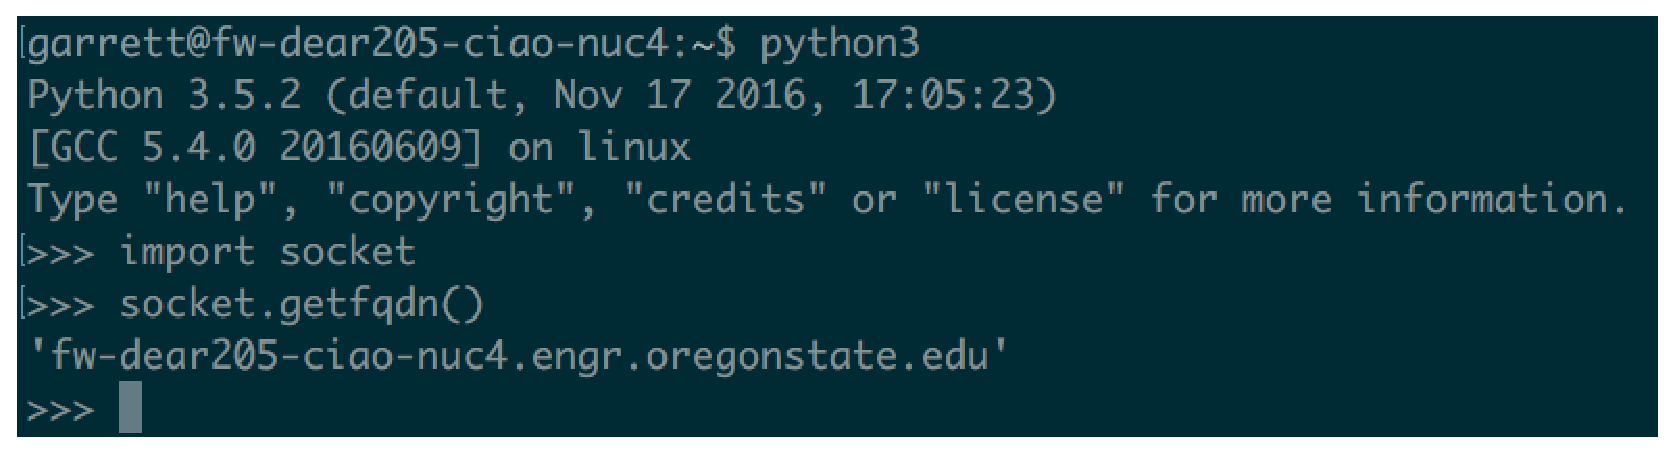
\includegraphics[scale=0.5]{getfqdn.eps}
\end{frame}

\begin{frame}
	\frametitle{Migrating to Ubuntu 16}
	We migrated to Ubuntu because of the issues with Docker certificates and
	\texttt{getfqdn()} on Clear Linux. Most of the Ciao team develops on
	Ubuntu.
\end{frame}

\begin{frame}
	\frametitle{Problems Running Workloads}
	\begin{itemize}
		\item After we set up Ciao, we ran into issues running workloads.
		\item When Ciao sets up a CNCI it uses DHCP to assign an IP address to it.
		\item OSU's network will not assign IP addresses to the CNCIs.
		\item To work around this we moved the Nucs off of OSU's network.
		\item We are running a DHCP server on the Cisco switch we are using for the LAN
	\end{itemize}
\end{frame}

\begin{frame}
	\frametitle{Open vSwitch}
	Goal: implement GRE tunnels with Open vSwitch by the end of week five

	This did not happen.
\end{frame}

\begin{frame}[allowframebreaks, fragile]
	\frametitle{Open vSwitch - libovsdb}
	It was originally our plan to implement with libovsdb.

	\begin{lstlisting}[caption=libovsdb insert operation]
	"op": "insert",
	"table": "Port",
	"row": <port information>,
	"type": "gre",
	"uuid-name": "uuid"
	\end{lstlsting}

	But! We actually need to create an OVS bridge for this to work.

\end{frame}

\begin{frame}[allowframebreaks, fragile]
	\frametitle{Open vSwitch - OVS bridge first}

	\begin{lstlisting}[caption=No Linux Bridge and OVS Tunnel]
		mrsj@singlevm:~\$ sudo brctl addbr br1
		mrsj@singlevm:~\$ sudo brctl show
		bridge name     bridge id               STP enabled     interfaces
		br0             8000.000000000000       no
		br1             8000.000000000000       no
		docker0         8000.02427ef725d4       no
		mrsj@singlevm:~\$ sudo ovs-vsctl add-port br1 gre0 -- set interface gre0 type=gre options:remote_ip=192.215.10.0
		ovs-vsctl: no bridge named br1
	\end{lstlsting}
\end{frame}

\begin{frame}
	\frametitle{Next Steps}
	Now our scope has changed a bit - we need to actually create bridges for
	the OVS tunnels to connect to.
\end{frame}

\begin{frame}
	\frametitle{References}
	\bibliographystyle{IEEEtran}
	\bibliography{pres}
\end{frame}

\end{document}
